\documentclass[11pt]{article}
\usepackage[margin=2.5cm]{geometry}
\usepackage[utf8]{inputenc}
\usepackage[T1]{fontenc}
\usepackage{amsmath}
\usepackage{array}
\usepackage{graphicx}

\title{Automatic Detection of Scoria Cones from DEMs}
\author{Gabriele Berruti (4791919)\\Computational Vision --- University of Genoa}
\date{}

\begin{document}
\maketitle

\section{Introduction}
This project detects \emph{scoria cones} from single-channel Digital Elevation
Models (DEMs), where each pixel encodes a terrain elevation in metres. The core
contribution is the \textbf{separation of nested or adjacent cones}: point-based
blob detectors collapse two overlapping craters into a single response, and a
one-to-one matching then discards one of the two. We address this with a
watershed segmentation of the crater depressions, which natively splits adjacent
catchment basins.

We work on three datasets: \textbf{El Hierro} (5\,m resolution, with ground-truth
annotations, used for development and validation), \textbf{Etna} (2\,m, noisier
ground truth, used as a stress test) and \textbf{Jeju} (10\,m, no ground truth,
used for qualitative and unsupervised analysis).

\section{Data and preprocessing}

\subsection{Step 0 --- DEM loading and inspection}
A DEM is a \emph{range image}: a single elevation band. Each dataset uses a
different \emph{nodata} sentinel, which we convert to \texttt{NaN} so that all
later computations ignore invalid pixels naturally. Table~\ref{tab:dems}
summarises the three DEMs after loading.

In Table~\ref{tab:dems}, $H\times W$ is the raster size in pixels (matrix rows
$\times$ columns), Mpx the total number of pixels in millions ($H\cdot W$, a proxy
for the memory footprint), Res. the ground size of one pixel in metres, dtype the
numeric type of the elevation values, and $z_{\max}$ the maximum elevation
(sanity check against the real volcano).

\begin{table}[h]
\centering
\begin{tabular}{l r r c c r}
\hline
Dataset & Size (H$\times$W) & Mpx & Res. (m) & dtype & $z_{\max}$ (m)\\
\hline
El Hierro & $5081\times5681$ & 28.9 & 5 & float32 & 1499.8\\
Etna      & $27756\times25717$ & 713.8 & 2 & float32 & 3324.1\\
Jeju      & $4364\times7761$ & 33.9 & 10 & float32 & 1945.0\\
\hline
\end{tabular}
\caption{DEM inspection. Maximum elevations match the real volcanoes
(Etna $\approx$3.3\,km, El Hierro $\approx$1.5\,km, Hallasan/Jeju
$\approx$1.95\,km), confirming correct loading.}
\label{tab:dems}
\end{table}

Three facts drive the following steps: (i) Etna is $\approx$714\,Mpx
($\approx$2.86\,GB as float32), so it must be processed in \emph{tiles} rather
than loaded whole; (ii) the three \emph{nodata} conventions differ
($-3.4\times10^{38}$, $-9999$, \texttt{NaN}) and are all mapped to \texttt{NaN};
(iii) each dataset has its own UTM coordinate reference system, so any shapefile
must be reprojected into the CRS of its DEM before use.

\subsection{Step 0.5 --- Visual inspection}
Before deriving any channel we inspect the data on El Hierro. Figure~\ref{fig:channels}
shows that the raw DEM looks visually flat, whereas the Eduard renderings (NE/NW shading
and texture shading) reveal the cones; this motivates the derived channels of Step~1.
Figure~\ref{fig:gt} shows the $196$ crater outlines of the ground truth: the two closest
craters lie only $25$\,m apart (5 pixels) and several cones are adjacent or nested.
Point-based blob detectors merge such pairs into a single detection --- separating them
is the goal of the watershed step.

For clarity, the panels in Figure~\ref{fig:channels} are: the \textbf{raw DEM}, i.e. the
original elevation grid where each pixel is a terrain height in metres (it looks flat
because a cone is only tens of metres tall relative to the whole island); the
\textbf{Eduard renderings}, relief-shaded views produced by the \emph{Eduard}
relief-shading tool and shipped with the dataset; the \textbf{NE/NW shading} (hillshade),
where the terrain is lit by a simulated sun from the North-East/North-West so that slopes
facing the light are bright and those facing away are dark (two opposite directions are
given so no slope stays in shadow); and the \textbf{texture shading}, a
light-direction-independent rendering that emphasises fine surface detail.

\begin{figure}[h]
\centering
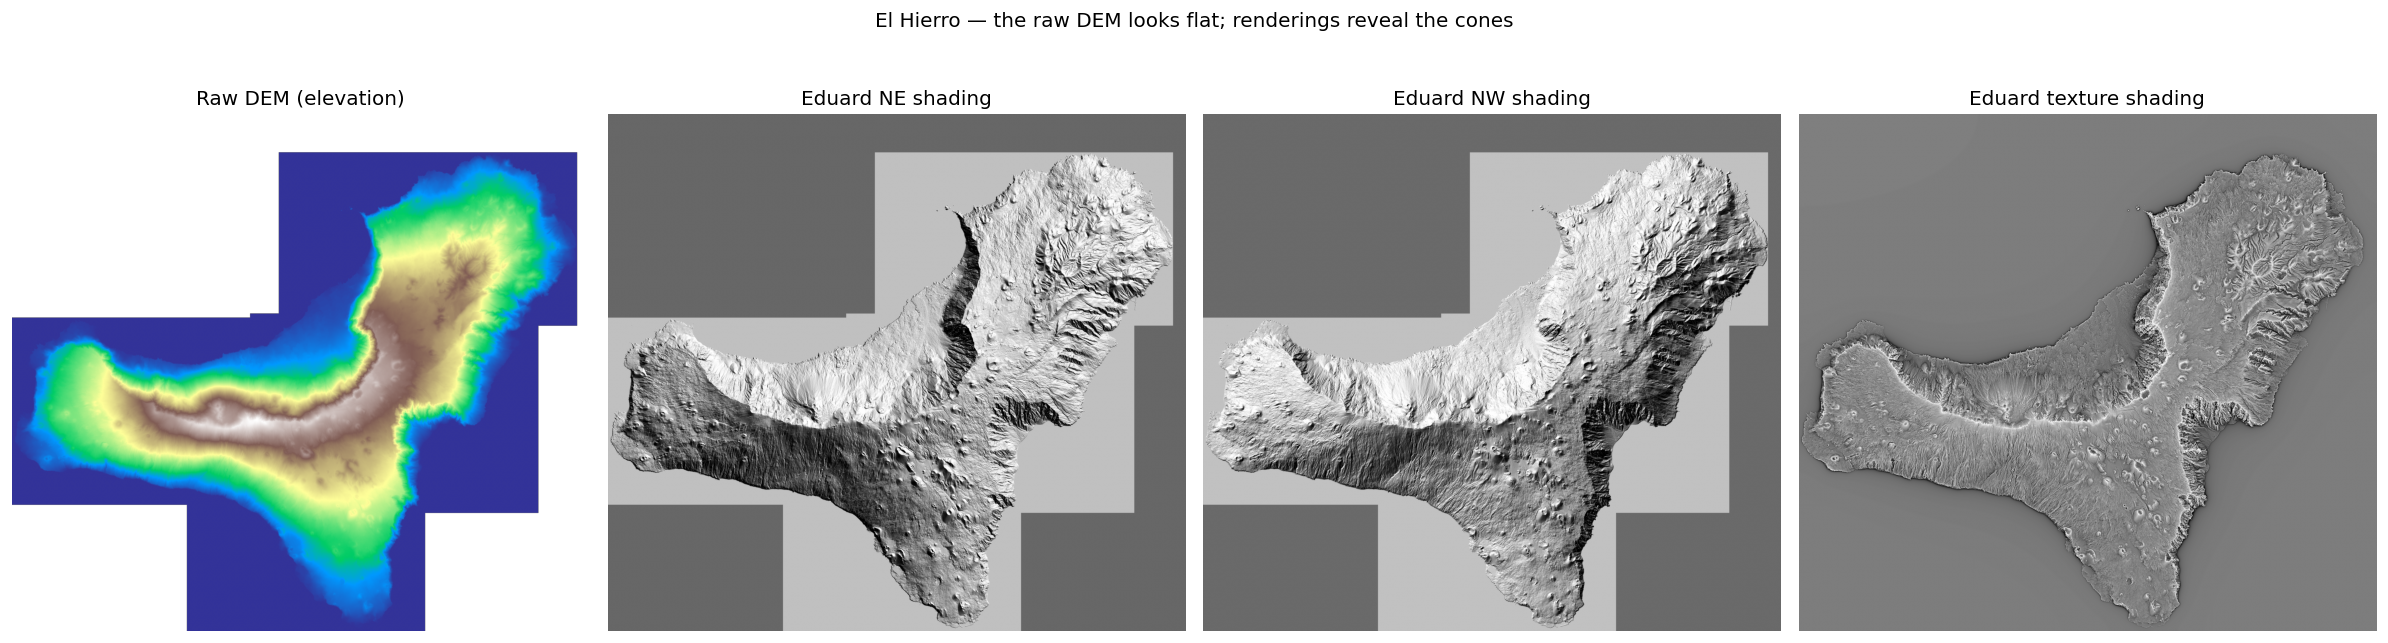
\includegraphics[width=\textwidth]{figures/fig_channels.png}
\caption{El Hierro: the raw DEM (left) is visually flat, while the Eduard renderings
reveal the conical landforms.}
\label{fig:channels}
\end{figure}

\begin{figure}[h]
\centering
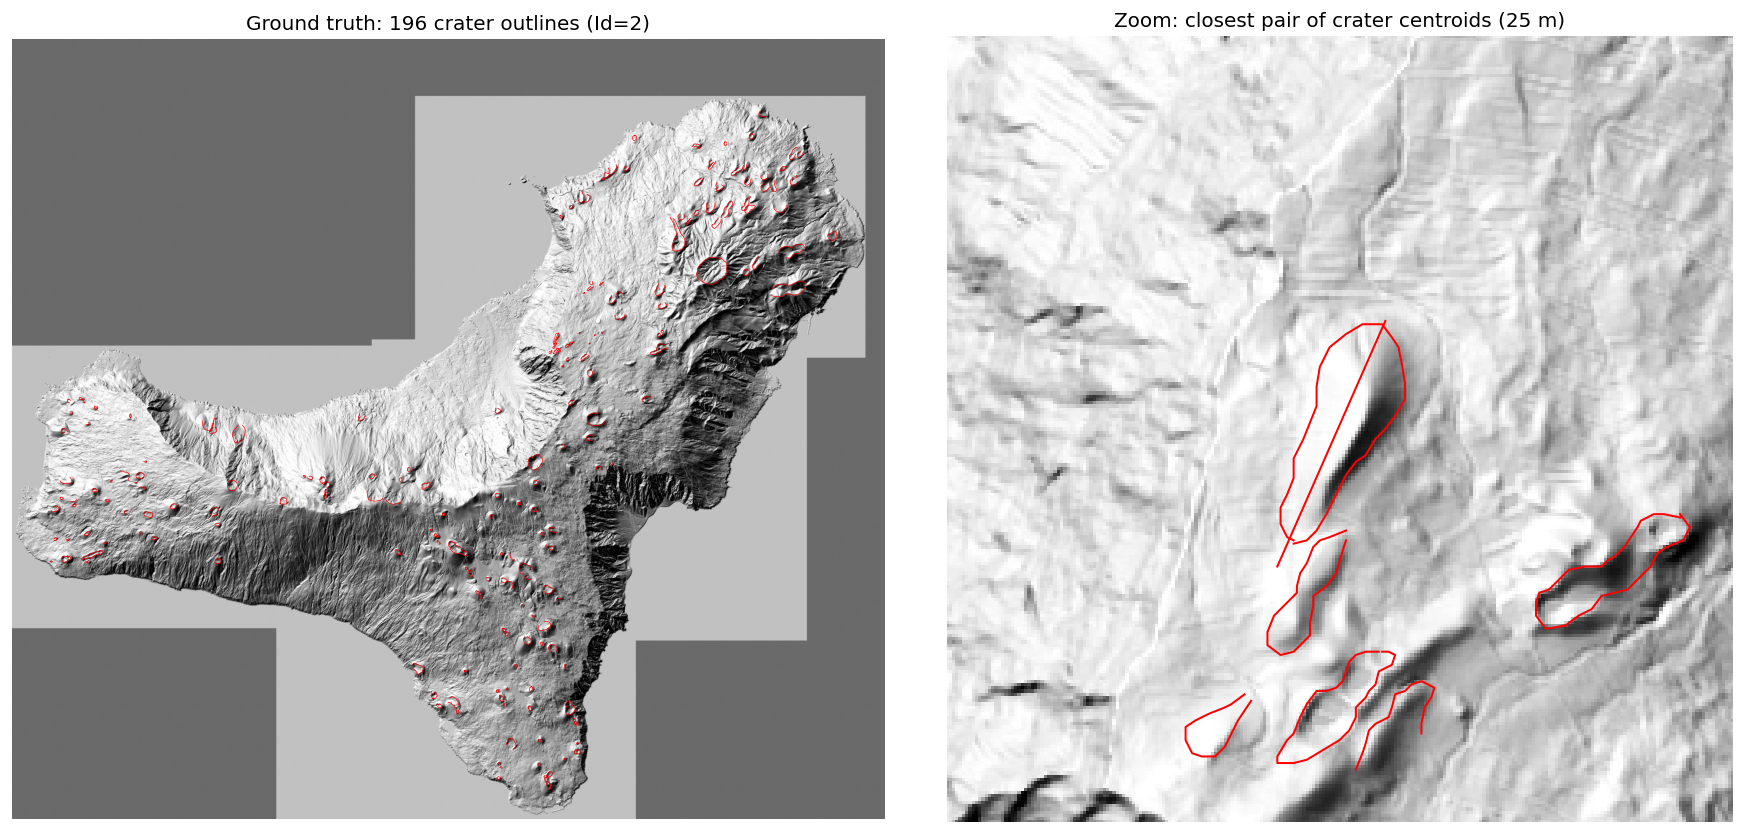
\includegraphics[width=\textwidth]{figures/fig_gt.png}
\caption{Ground truth on El Hierro. Left: the 196 crater outlines (Id$=2$). Right: a
zoom on the closest pair of crater centroids ($25$\,m apart).}
\label{fig:gt}
\end{figure}

Figure~\ref{fig:adjacent} isolates the cones that actually \emph{overlap}, i.e. whose
nearest neighbour is closer than the sum of the two radii. These are $8$ craters in $4$
pairs; note that they are not the single closest centroids of Figure~\ref{fig:gt} (two
small craters), but pairs of \emph{large} adjacent cones whose outlines intersect. These
are the configurations a point-based detector merges into one and the watershed step must
separate.

\begin{figure}[h]
\centering
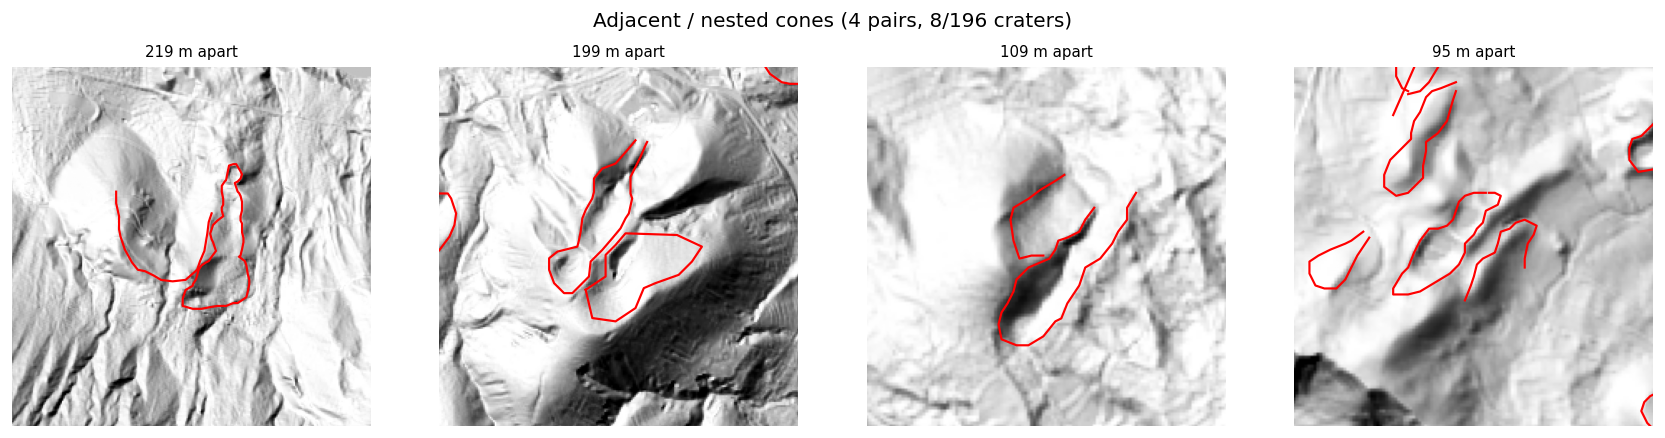
\includegraphics[width=\textwidth]{figures/fig_adjacent.png}
\caption{The adjacent/nested cases on El Hierro: the 4 crater pairs whose outlines
overlap (8 craters). The watershed step is designed to split exactly these.}
\label{fig:adjacent}
\end{figure}

\paragraph{Ground-truth quality and label semantics.}
The El Hierro shapefile is \emph{dirty} and mixes three feature types in a single file.
The crater outlines (Id$=2$) are open polylines: $191$ of $196$ do not close (median
start--end gap $40$\,m, up to $556$\,m) and some have as few as $2$ vertices. We therefore
use crater \emph{centroids} (plus an approximate radius) rather than the exact outline
shape. A geometry test then characterises the three labels (Table~\ref{tab:labels}):
Id$=1$ is the cone \textbf{base} (large, round, and enclosing the crater in $98\%$ of
cones), Id$=2$ the \textbf{crater} rim, and Id$=3$ a \textbf{fissure} --- a short, strongly
elongated segment that always carries a non-zero azimuth in the \texttt{Prj\_Az} field.
The \texttt{pericolosi} field is a hazard level ($0/1/2$). We adopt Id$=2$ as the detection
target.

\begin{table}[h]
\centering
\begin{tabular}{c l r r r r c}
\hline
Id & meaning & n & verts & length (m) & aspect & Prj\_Az$\neq 0$\\
\hline
1 & base    & 151 & 29 & 846 & 1.29 & 0\%\\
2 & crater  & 196 & 19 & 457 & 1.47 & 0\%\\
3 & fissure & 171 & 2  & 272 & 8.32 & 100\%\\
\hline
\end{tabular}
\caption{Data-driven characterisation of the El Hierro labels (median values). The high
aspect ratio and the always-present azimuth identify Id$=3$ as fissures.}
\label{tab:labels}
\end{table}

\subsection{Step 0.6 --- Quick data analysis}
Three cheap measurements on El Hierro parameterise the later steps rather than guessing
their constants. (i) The three Eduard renderings share the DEM grid exactly (same
$5081\times5681$ shape and transform), so overlays are pixel-exact. (ii) The equivalent
radius of the crater outlines (Figure~\ref{fig:stats}, left) has median $71$\,m and a
5th--95th percentile range of $20$--$174$\,m, which we adopt as the LoG detector scale
range. (iii) The nearest-neighbour distance between craters (Figure~\ref{fig:stats},
right) has median $418$\,m but a minimum of $25$\,m, and $8/196$ craters ($4\%$) lie
closer to a neighbour than the sum of the two radii, i.e. they are adjacent or nested.
This $4\%$ is precisely the population that point-based detection merges and that the
watershed step is designed to recover.

\begin{figure}[h]
\centering
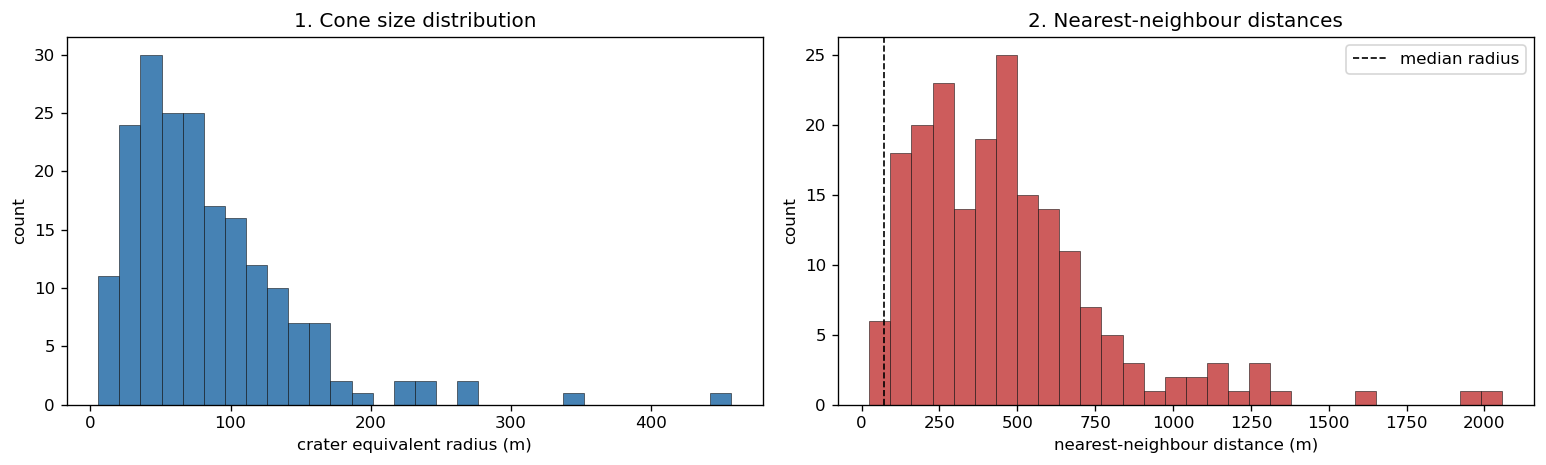
\includegraphics[width=\textwidth]{figures/fig_data_stats.png}
\caption{El Hierro crater statistics. Left: equivalent-radius distribution, used to set
the LoG scale range. Right: nearest-neighbour distance distribution; the dashed line is
the median radius, and the cones below it are the adjacent/nested cases.}
\label{fig:stats}
\end{figure}

\section{Detection pipeline}

\subsection{Step 1 --- Morphometric channels}
From the single elevation band we derive three channels with the image gradient
(deck \texttt{01\_image\_processing}, p.13): the \textbf{slope}
$=\arctan\sqrt{g_x^2+g_y^2}$ in degrees, the \textbf{aspect}
$=\operatorname{atan2}(g_y,g_x)$ (the direction the slope faces), and the
\textbf{roughness}, the local standard deviation of elevation in a $5\times5$ window.
Figure~\ref{fig:morpho} shows them on El Hierro. As a quantitative check, the median slope
on the crater rims is $18.8^\circ$ against $8.1^\circ$ on the background (about
$2.3\times$ steeper), and the aspect rotates around each cone, giving the radial pattern of
the rightmost panel. These three channels, together with the texture rendering, are the
input of the detection steps.

\begin{figure}[h]
\centering
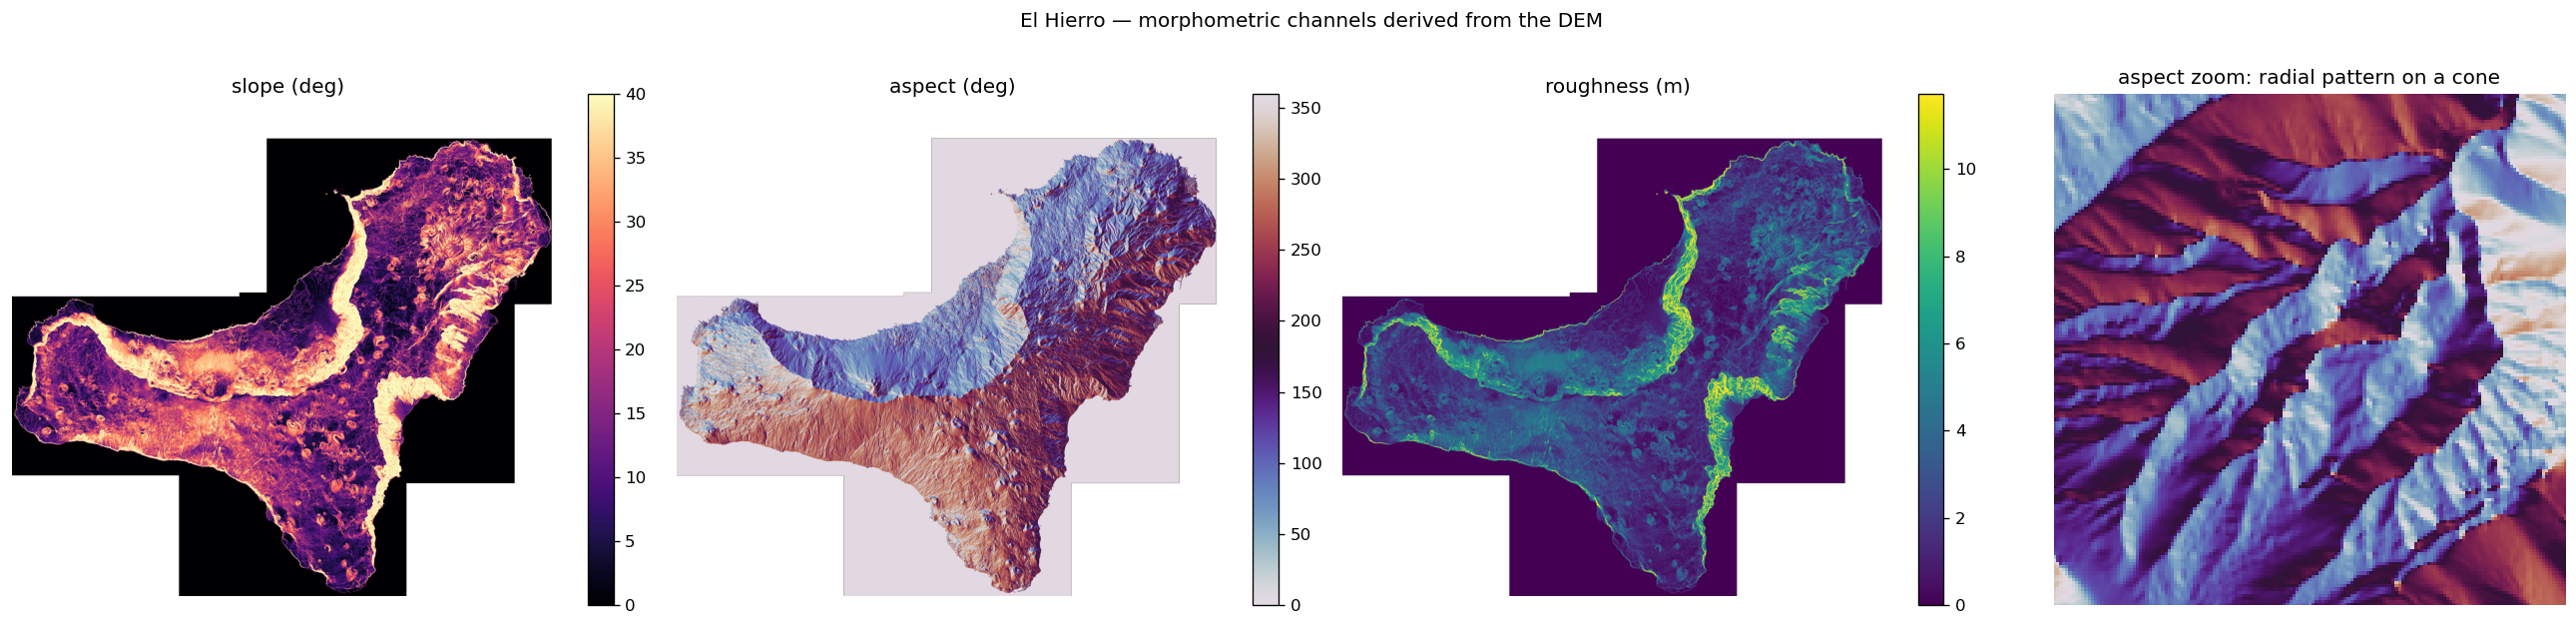
\includegraphics[width=\textwidth]{figures/fig_morphometric.png}
\caption{Morphometric channels derived from the El Hierro DEM: slope, aspect and roughness,
plus a zoom of the aspect showing the radial pattern around a single cone.}
\label{fig:morpho}
\end{figure}

\end{document}
